\section{Bericht}

\subsection{Einleitung}
Ziel der Übung ist es mit Hilfe von Xcos eine Simulation des Balles auf einer geneigten Fläche aufzubauen. Dazu muss das Script aus \textit{Labor 1} simuliert werden. Zur Regelung des Servo-Motors wird ein PID-Regler benutzt. Des weiteren ist es Teil der Übung, eine Jumping Reference mit einzubauen, um alle zehn Sekunden den Referenzwert für den Ball aus einem gegebenen Intervall zu verändern.

\subsection{Durchführung}
Zuerst haben wir ein Grundgerüst der Simulation basierend auf \textit{Abbildung 1} aus der Aufgabenstellung gebaut. Wir haben uns dazu entschieden nicht nur das BOIP-Modell in einen einzelnen Super-Block zu packen, sondern auch den PID-Regler. Die gesamte Simulation kann in vier Teile zerlegt werden (BOIP-Modell, PID-Regler, Berechnung der Position, Jumping Reference). Diese werden im Folgenden beschrieben.

\subsubsection{BOIP-Modell}
Im Super-Block für das BOIP-Modell haben wir das Skript aus \textit{Labor 1} mit Hilfe von Blöcken nachgebaut. Neben Konstanten und mathematischen Operations-Blöcken verwenden wir zur Simulation auch Bedingungen und Begrenzungen. Der Eingang des Super-Blocks ist $\beta$, der Ausgang $\alpha$. \\
Das Eingangssignal wird mit einem Saturation-Block auf den für uns relevanten Bereich $\beta = \pm 40 ^\circ$ begrenzt. Anschließend werden wie in \textit{Labor 1} die Werte für $\gamma_1$, $c_1$, $\beta_2$ und $\alpha_1$ berechnet. Um abschließend $\alpha$ zu berechnen muss $\beta$ mit $\gamma$ verglichen werden. Wenn $\beta \geq \gamma$ ist, wird $\alpha_1$ positiv, im Fall $\beta < \gamma$ negativ eingerechnet. Diesen Vergleich haben wir mit einem If-Then-Else-Block und einem Selector umgesetzt. Somit erhalten wir letztendlich den Wert $\alpha$ als Ausgabe des Super-Blocks.

\subsubsection{PID-Regler}
Der PID-Regler simuliert den Servo-Motor des Modells. Die Eingabe in diesen Super-Block ist der Fehlerwert, die Ausgabe der Winkel $\beta$. \\
Der Regler besteht aus drei Berechnungsabschnitten, deren Resultate am Ende addiert werden. Durch Annäherung sind wir auf die Werte \textit{3,5} für den P-Teil, \textit{1,45} für den I-Teil und \textit{2,7} für den D-Teil gekommen. Wir haben versucht einen Tiefpass-Filter einzubauen, jedoch hat dieser unser Resultat nur verschlechtert, weshalb wir diesen wieder verwarfen.

\subsubsection{Berechnung der Position}
Die Berechnung der Position basiert auf der Formel $ x = \iint \frac{5}{7} \cdot g \cdot sin(\alpha) \cdot d t^2 $ aus der Aufgabenstellung von \textit{Labor 1}. Diese haben wir mit Hilfe von einer Konstanten, einem Mulitplikations-Block, zwei Integrations-Blöcken sowie einem Sinus-Block modelliert. Den Winkel $\alpha $ nehmen wir direkt aus dem Ausgang des BOIP-Super-Blocks. Vor dem ersten Integral finden wir den Wert der Beschleunigung, nach dem ersten Integral den Wert der Geschwindigkeit und nach dem zweiten Integral die Position. Diese wird zum Anfang zurückgeführt, um den Fehlerwert zu berechnen.

\subsubsection{Jumping Reference}
Eine weitere Aufgabe war es, eine Jumping Reference einzubauen, die einen Referenzwert aus einem gegebenen Intervall für zehn Sekunden hält und dann auf einen anderen Wert springt. Dabei soll immer zwischen positiven und negativen Werten gewechselt werden. \\
Unsere Jumping Reference wählt immer einen vor drei vorgegebenen Werten, wobei jeder zweite gewählte Wert negativ ist. \\
\begin{center}
	\begin{minipage}{\linewidth}
	\centering
	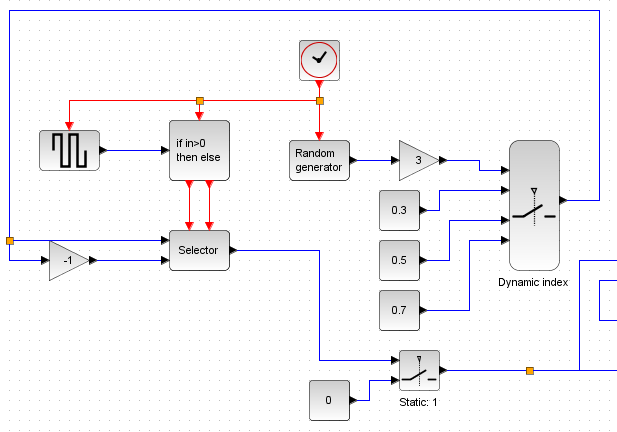
\includegraphics[scale=0.7]{images/jumping_reference.png}
	\captionof{figure}{Jumping Reference und statischer Wert}
	\end{minipage}
\end{center}

In unserer Simulation ist es möglich zwischen einem fest vorgegebenen Sollwert und der Jumping Reference zu wechseln.

\subsection{Ergebnis}

\begin{center}
	\begin{minipage}{\linewidth}
	\centering
	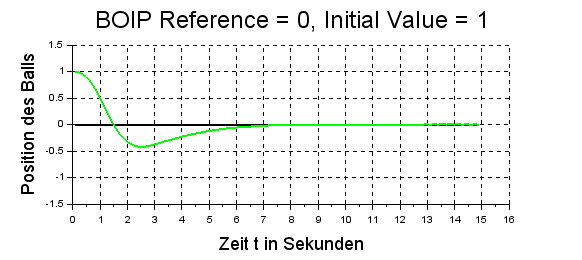
\includegraphics[scale=0.7]{images/ref0_init1.png}
	\captionof{figure}{Simulation 1}
	\end{minipage}
\end{center}
In unserem ersten Versuch haben wir den Referenzwert auf \textit{0} gesetzt und den Initialwert des Balls auf \textit{1}. Man sieht das der Ball nach ungefähr \textit{7,5} Sekunden an der gewünschten Position liegen bleibt. Der PID-Regler ist so eingestellt, dass er einmal kurz über schwingt und sich dann der Soll-Position nähert. Das Überschwingen wird durch den hohen P-Anteil erklärt.\\ \\

\begin{center}
	\begin{minipage}{\linewidth}
	\centering
	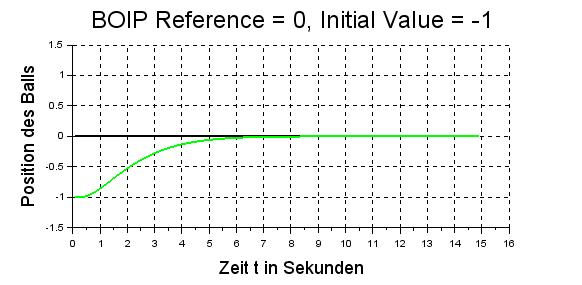
\includegraphics[scale=0.7]{images/ref0_init-1.png}
	\captionof{figure}{Simulation 2}
	\end{minipage}
\end{center}
In \textit{Abbildung 3} ist der Referenzwert auf \textit{0} gesetzt, der Initialwert auf \textit{-1}. Hier nähert sich der Ball langsam dem eingestellten Sollwert ohne ein Überschwingen und erreicht diesen nach ungefähr \textit{8,5} Sekunden. \\ \\

\begin{center}
	\begin{minipage}{\linewidth}
	\centering
	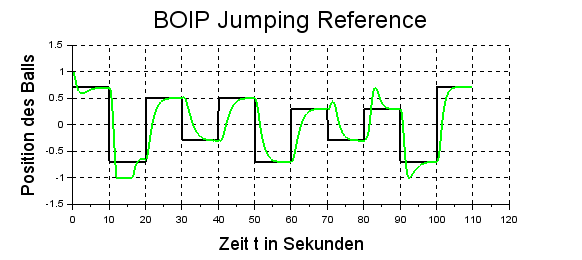
\includegraphics[scale=0.7]{images/jumpingref.png}
	\captionof{figure}{Simulation 3}
	\end{minipage}
\end{center}
In \textit{Abbildung 4} ist unser letzter Versuch dargestellt. Der Referenzwert wird alle zehn Sekunden auf einen von drei vorgegebenen Werten gesetzt. Außerdem ist jeder zweite Wert negativ.\\
Man sieht, dass der Ball allerdings nicht bei jedem Wechsel schnell genug an der gewünschten Stelle liegen bleibt. Wir haben lange versucht dieses Problem durch Veränderungen am PID-Regler zu lösen, dies ist uns jedoch leider nicht gelungen.


\subsection{Fazit}
Bei einem fest vorgegebenen Wert ist es uns gelungen, den Ball in unter zehn Sekunden an die gewünschte Position zu manövrieren. \\
Wird der feste Wert durch eine Jumping Reference ersetzt, gelingt uns dies jedoch nicht immer, da der Regler manchmal zu langsam ist.\\
Selbst nach sehr langer Bearbeitungszeit war es uns nicht möglich ein für uns zufriedenstellendes Ergebnis zu erreichen. Wie zu sehen ist, treten die Referenzwerte nicht immer schnell genug oder sogar gar nicht ein. Für dieses Problem haben wir keine Lösung gefunden.